% !TeX root = ./eLife_draft.tex

%%%%%%%%%%%%%%%%%%%%%%%%%%%%%%%%%%%%%%%%%%%%%%%%%%%%%%%%%%%%
%%% ELIFE ARTICLE TEMPLATE
%%%%%%%%%%%%%%%%%%%%%%%%%%%%%%%%%%%%%%%%%%%%%%%%%%%%%%%%%%%%
%%% PREAMBLE 
\documentclass[9pt,lineno]{elife}
% Use the onehalfspacing option for 1.5 line spacing
% Use the doublespacing option for 2.0 line spacing
% Please note that these options may affect formatting.
% Additionally, the use of the \newcommand function should be limited.

\usepackage{lipsum} % Required to insert dummy text
\usepackage[version=4]{mhchem}
\usepackage{siunitx}
\DeclareSIUnit\Molar{M}

%%%%%%%%%%%%%%%%%%%%%%%%%%%%%%%%%%%%%%%%%%%%%%%%%%%%%%%%%%%%
%%% ARTICLE SETUP
%%%%%%%%%%%%%%%%%%%%%%%%%%%%%%%%%%%%%%%%%%%%%%%%%%%%%%%%%%%%

\title{Fundamental limits on the rate of bacterial cell division}
\author[1, *]{Nathan M. Belliveau}
\author[2, 3, *]{Griffin Chure}
\author[4]{Christina L. Hueschen}
\author[5]{Hernan G. Garcia}
\author[6]{Jan\'{e} Kondev}
\author[7]{Daniel S. Fisher}
\author[1, 8]{Julie Theriot}
\author[1, 9, $\dagger$]{Rob Phillips}
\affil[1]{Department of Biology, University of Washington, Seattle, WA, USA}
\affil[2]{Division of Biology and Biological Engineering, California Institute of Technology, Pasadena, CA, USA}
\affil[3]{Department of Applied Physics, California Institute of Technology, Pasadena, CA, USA}
\affil[4]{Department of Chemical Engineering, Stanford University, Stanford, CA, USA}
\affil[5]{Department of Molecular Cell Biology and Department of Physics, University of California Berkeley, Berkeley, CA, USA}
\affil[6]{Department of Physics, Brandeis University, Waltham, MA, USA}
\affil[7]{Department of Applied Physics, Stanford University, Stanford, CA, USA}
\affil[8]{Allen Institute for Cell Science, Seattle, WA, USA}
\affil[9]{Department of Physics, California Institute of Technology, Pasadena, CA, USA}
\affil[$\dagger$]{Address correspondence to phillips@pboc.caltech.edu}
\affil[*]{Contributed equally}

\contrib[$\dagger$]{These authors contributed equally to this work}

%%%%%%%%%%%%%%%%%%%%%%%%%%%%%%%%%%%%%%%%%%%%%%%%%%%%%%%%%%%%
%%% ARTICLE START
%%%%%%%%%%%%%%%%%%%%%%%%%%%%%%%%%%%%%%%%%%%%%%%%%%%%%%%%%%%%

\begin{document}

\maketitle

\begin{abstract}

\end{abstract}

% !TeX root = ./eLife_draft.tex

\section{Introduction}
The observed range of bacterial growth rates is enormously diverse. In natural
environments, some microbial organisms may double only once per year
\citep{mikucki2009} while in comfortable laboratory conditions, growth can be
rapid with several divisions per hour \citep{schaechter1958}. This six
order-of-magnitude difference in time scales of growth encompasses different
microbial species and lifestyles, yet even for a single species such as
\textit{Escherichia coli}, the growth rate can be modulated over a
large scale by tuning the type and amount of nutrients in the growth medium
\citep{liu2005a}. This remarkable plasticity in growth rate illustrates the
intimate relationship between environmental conditions and the rates at which
cells convert nutrients into new cellular material -- a relationship that has
remained a major topic of inquiry in bacterial physiology for over a century
\citep{jun2018}.

A key discovery in bacterial physiology of the past 70 years was the
identification of bacterial "growth laws" \citep{schaechter1958}; empirical
relationships that relate the bacterial growth rate to the protein and RNA
composition of the intracellular milieu in a number of different species.
Over the past decade, a flurry of work \citep{molenaar2009, scott2010,
klumpp2014, basan2015, dai2016, erickson2017} has examined these growth laws
at a quantitative level, developing a series of phenomenological models from
which the growth laws naturally emerge. In parallel, a "molecular revolution"
in biology has yielded an increasingly refined molecular census of the cell,
particularly for bacteria such as the microbial workhorse \textit{E. coli}
\citep{schmidt2016, davidi2016a}. In light of the now expansive trove of
quantitative biological data, we can revisit several of the evergreen
questions about bacterial growth and physiology that were originally raised
by microbiologists in the middle of the 20th century. Specifically, what
biological processes are the primary determinants for how quickly bacterial
cells can grow and reproduce? Why do cells modulate the absolute numbers and
relative ratios of their molecular constituents as a function of changes in
growth rate or nutrient availability?

In this work, we begin by considering these two questions from two distinct
angles. First, as a result of an array of high-quality proteome-wide
measurements of \textit{E. coli} under diverse growth conditions, we have
generated a census that allows us to explore how the number of key molecular
players change as a function of growth rate. Here, we have assembled a singular
data set of protein copy numbers using measurements collected over the past
decade via mass spectrometry \citep{schmidt2016, peebo2015, valgepea2013} or
ribosomal profiling \citep{li2014} of the composition of the \textit{E. coli}
proteome across a gamut of growth rates. Due to notable changes in cell size and
cellular composition as a function of growth rate \citep{bremer2008,
taheriaraghi2015}, as well as differences in normalization and standardization
schemes used in each experimental work, substantial care was taken to ensure
consistency on a per cellular basis (see the Appendix for a detailed analysis
and additional discussion). To our knowledge, this compiled and curated dataset
represents the most comprehensive view to date of the \textit{E. coli} proteome,
covering $\approx$ 4000 proteins and 36 unique growth rates, with the observed
abundance of any given protein being directly comparable between data sets and
across growth rates. This allows us to interrogate  the \textit{E. coli}
specific physiology underlying the observed abundances while  minimizing the
effects of experimental noise, as  $\approx$ 75\% of the  proteins are observed
in at least two separate datasets.

Second, by compiling molecular turnover rate measurements for many of the
fundamental processes associated with bacterial growth, we make quantitative
estimates of a handful of key cellular processes (schematized in
\FIG{categories}) to determine whether our current understanding of the
kinetics of these processes are sufficient to explain the magnitude of the
observed protein copy numbers across conditions (see \BOX{estimate_rules}
describing the philosophy behind this approach). The census, combined with
these estimates, provide a window into the question of whether the rates of
central processes such as energy generation or DNA synthesis vary
systematically as a function of cell growth rate by altering protein copy
number.

Throughout our estimates, we consider an archetypal growth rate of $\approx$
0.5 hr$^{-1}$ corresponding to a doubling time of $\approx$ 5000 seconds, as
the data sets examined here heavily sample this growth regime. While we
formulate point estimates for the protein abundances at this division time,
we also consider how these values will vary at other growth rates due to
changes in cell size, surface area, and chromosome copy number
\citep{taheriaraghi2015, harris2018}. For the majority of the processes
considered, we find that the protein copy numbers appear tuned for the task
of cell doubling across a continuum of growth rates. Thus, our understanding
of the kinetics of various biological processes is sufficient to
quantitatively explain the observed abundances of these proteins.

% From these estimates, it emerges that translation, particularly the synthesis of
% ribosomal proteins, is a plausible candidate that limits the rate of cellular
% growth in \textit{E. coli}.

From these estimates, it emerges that translation,  particularly the synthesis of ribosomal proteins is a
plausible candidate that limits the rate of cellular growth in \textit{E. coli}.
We reach this conclusion by considering that ribosome synthesis is 1) a rate
limiting step for the \textit{fastest} bacterial division, and  2) the main
determinant of bacterial growth rate across  nutrient conditions associated with
moderate to fast growth rates. In addition, a strict dependence between the
maximal growth rate and ribosomal mass fraction coincides with the regime where
the growth laws appear most valid \citep{amir2017, scott2010}. This enables us
to suggest that the long-observed correlation between growth rate and cell size
\citep{schaechter1958, si2017} can be simply attributed to the increased
absolute number of ribosomes per cell under conditions supporting extremely
rapid growth. To better understand how the observed alterations in absolute
protein abundances, and in particular, changes in ribosome copy number,
influence growth rate across different nutrient conditions we consider a minimal
model of cellular growth. Our conclusions from these analyses provide important
insight into how \textit{E. coli} regulates growth across conditions of
differing nutrient availability and identifies fundamental constraints in
bacterial growth more broadly.






\begin{figure}
    \centering{
    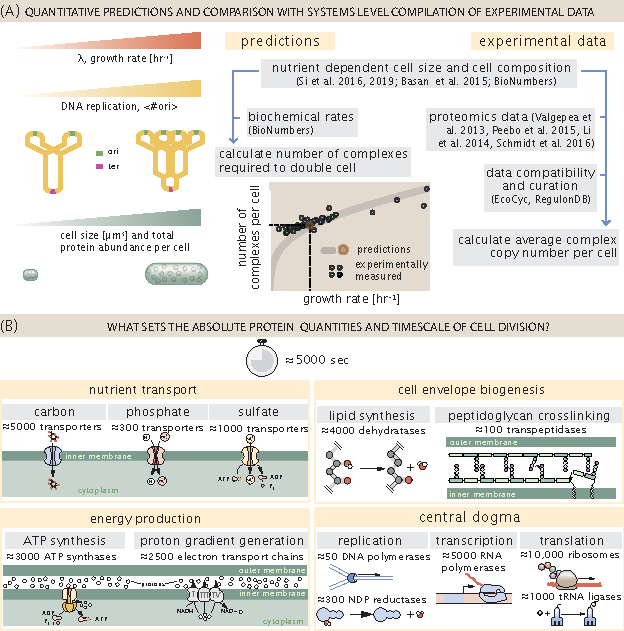
\includegraphics{main_figs/fig1_schematic_categories_grouped.pdf}
    \caption{\textbf{Transport and synthesis processes necessary for cell division.}
            We consider an array of processes necessary for a cell to double its
            molecular components, broadly grouped into four classes. These
            categories are (A) nutrient transport across the cell membrane, (B) cell envelope
            biogenesis, (C) energy production (namely, ATP synthesis), and (D) processes associated with the central dogma.
            Numbers shown are the approximate number of complexes of each type
            observed at a growth rate of 0.5 hr$^{-1}$, or a cell doubling time
            of $\approx$ 5000 s.}
    \label{fig:categories}
    }
\end{figure}

% \section{Nutrient Transport}
In order to build new cellular mass, the molecular and elemental building
blocks must be scavenged from the environment in different forms. Carbon, for
example, is acquired via the transport of carbohydrates and sugar alcohols
with some carbon sources receiving preferential treatment in their
consumption \citep{monod1947}. Phosphorus, sulfur, and nitrogen, on the other
hand, are harvested primarily in the forms of inorganic salts, namely
phosphate, sulfate, and ammonia \citep{jun2018, assentoft2016, stasi2019,
antonenko1997, rosenberg1977, willsky1973}. All of these compounds have
different permeabilities across the cell membrane and most require some
energetic investment either via ATP hydrolysis or through the proton
electrochemical gradient to bring the material across the hydrophobic cell
membrane. Given the diversity of biological transport mechanisms and the vast
number of inputs needed to build a cell, we begin by considering transport of
elemental requirements as a possible rate-limiting step of bacterial cell
division.


The elemental composition of \textit{E. coli} has received much quantitative
attention over the past half century \citep{neidhardt1991, taymaz-nikerel2010,
heldal1985, bauer1976}, providing us a starting point for estimating the
copy numbers of various transporters. While there is some variability in the
exact elemental percentages (with different uncertainties), we can estimate that the
dry mass of a typical \textit{E. coli} cell is $\approx$ 45\% carbon (BNID:
100649, \cite{milo2010}), $\approx$ 15\% nitrogen (BNID: 106666,
\cite{milo2010}), $\approx$ 3\% phosphorus (BNID: 100653, \cite{milo2010}), and
1\% sulfur (BNID: 100655, \cite{milo2010}). In the coming paragraphs, we will examine how many transporters and/or channels
must be present to maintain these elemental compositions with a moderate
doubling time of 6000 s.

\subsection{Carbon Transport}
We begin with the most abundant element by mass, carbon. Using $\approx$ 0.3
pg as the typical \textit{E. coli} dry mass (BNID: 103904, \cite{milo2010}),
we estimate that $\approx 10^{10}$ carbon atoms must be brought into the cell
in order to double all of the carbon-containing molecules (\FIG{carbon_tport}(A,
top))). Typical laboratory
growth conditions, such as those explored in the aforementioned proteomic data
sets, provide carbon as single class of sugar such as glucose, galactose, or
xylose to name a few. \textit{E. coli} has evolved myriad mechanisms by which these sugars can
be transported across the cell membrane. One such mechanism of transport is via
the PTS system which is a highly modular system capable of transporting a diverse
range of sugars \citep{escalante2012}. The glucose-specific
component of this system transports $\approx$ 200 glucose
molecules per second per channel (BNID: 114686, \cite{milo2010}). Making the
assumption that this is a typical sugar transport rate, coupled with the
need to transport 10$^{10}$ carbon atoms, we arrive at the conclusion that on the
order of 1000 transporters must be expressed in order to bring in enough carbon
atoms to divide in 6000 s, diagrammed in the top panel of \FIG{carbon_tport}(A). This estimate, along with the observed average number
of carbohydrate transporters present in the proteomic data sets
\citep{schmidt2016, peebo2015,valgepea2013,li2014}, is shown in
\FIG{carbon_tport}(A). While we estimate 1000 transporters are needed, the
data reveals that at a division time of $\approx 6000$ s there is nearly a
ten-fold excess of transporters. Furthermore, the data illustrates that the
average number of carbohydrate transporters present is largely-growth rate
independent.

\begin{figure}
    \begin{fullwidth}
    \centering{
    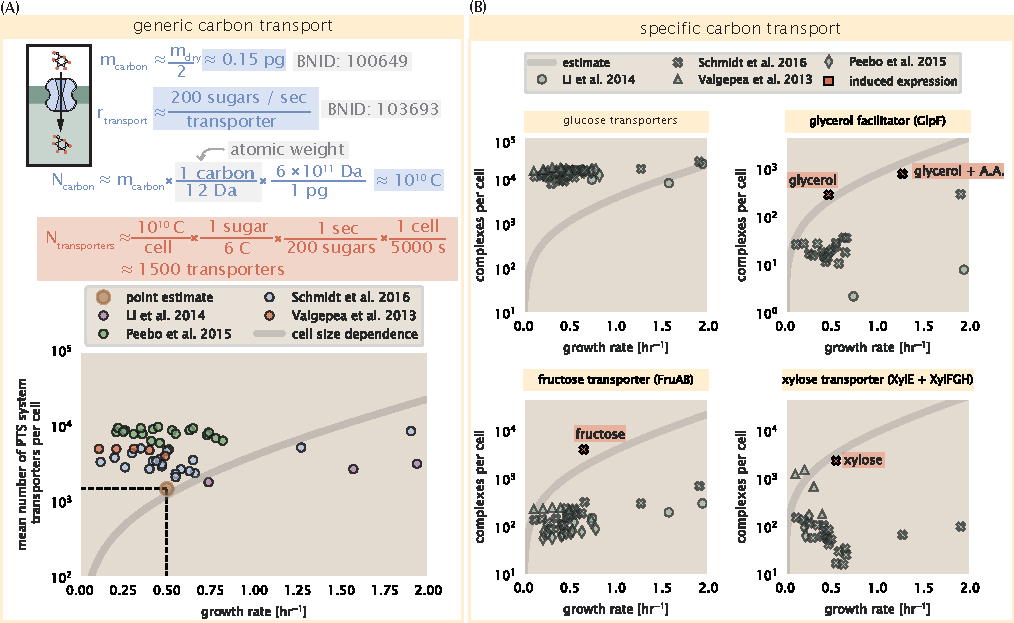
\includegraphics{main_figs/fig2_carbon_transport.pdf}
    \caption{\textbf{The abundance of carbon transport systems across growth
    rates.} (A) A simple estimate for the minimum number of generic carbohydrate
    transport systems (top) assumes $\approx 10^{10}$ C are needed to complete
    division, each transported sugar contains $\approx 6$ C, and each
    transporter conducts sugar molecules at a rate of $\approx 200$ per second.
    Bottom plot shows the estimated number of transporters needed at a growth
    rate of $\approx 0.5 $ per hr (light-brown point and dashed lines). Colored
    points correspond to the mean number of carbohydrate transporters for
    different growth conditions across different published datasets. (B) The
    abundance of various specific carbon transport systems plotted as a function
    of the population growth rate. Red points and red-highlighted text indicate conditions in which the
    only source of carbon in the growth medium induces expression of the
    transport system.}
    \label{fig:carbon_tport}
    }
    \end{fullwidth}
\end{figure}

The estimate presented in \FIG{carbon_tport}(A) neglects any specifics of the
regulation of carbon transport system and presents a data-averaged view of how
many carbohydrate transporters are present on average. Using the diverse array
of growth conditions explored in the proteomic data sets, we can explore how
individual carbon transport systems depend on the population growth rate. In
\FIG{carbon_tport}(B), we show the total number of carbohydrate transporters
specific to different carbon sources. A striking observation, shown in the
top-left plot of \FIG{carbon_tport}(B), is the constancy in the expression of the
glucose-specific transport systems (the PtsG enzyme of the PTS system and the
glucose-transporting ManXYZ complex). Additionally, we note that the total number
of glucose-specific transporters is tightly distributed $\approx 10^4$ per cell,
an order of magnitude beyond the estimate shown in \FIG{carbon_tport}(A). This
illustrates that \textit{E. coli} maintains a substantial number of complexes
present for transporting glucose which is known to be the preferential carbon
source \citep{monod1947, liu2005a, aidelberg2014}.

It is now understood that a large number of metabolic operons are regulated
with dual-input logic gates that are only expressed when glucose
concentrations are low (mediated by cyclic-AMP receptor protein CRP) and the
concentration of other carbon sources are elevated \citep{gama-castro2016, zhang2014a}. A
famed example of such dual-input regulatory logic is in the regulation of the
\textit{lac} operon which is only natively activated in the absence of glucose and the
presence of allolactose, an intermediate in lactose metabolism \citep{jacob1961}, though
we now know of many other such examples \citep{ireland2020, gama-castro2016,
belliveau2018}. This illustrates that once glucose is depleted from the
environment, cells have a means to dramatically increase the abundance of the
specific transporter needed to digest the next sugar that is present. Several
examples of induced expression of a specific carbon-source transporters are
shown in \FIG{carbon_tport}(B). Points colored in red (labeled by red
text-boxes) correspond to growth conditions in which the specific carbon source
(glycerol, xylose, or fructose) is present. These plots show that, in the
absence of the particular carbon source, expression of the transporters is
maintained on the order of $\sim 10^2$ per cell. However, when induced, the
transporters become highly-expressed and are present on the order of $\sim
10^4$ per cell, which exceeds the generic estimate given in
\FIG{carbon_tport}(A). Together, this generic estimation and the specific
examples of induced expression suggest that transport of carbon across the cell
membrane, while critical for growth, is not the rate-limiting step of cell division.

\subsection{Phosphorus and Sulfur Transport}
We now turn our attention towards other essential elements, namely phosphorus and
sulfur. Phosphorus is critical to the cellular energy economy in the form of
high-energy phosphodiester bonds making up DNA, RNA, and the XTP energy pool as
well as playing a critical role in the post-translational modification of
proteins and defining the polar-heads of lipids. In total, phosphorus
makes up $\approx$3\% of the cellular dry mass which in typical experimental conditions is in the form of inorganic phosphate. The cell membrane
has remarkably low permeability to this highly-charged and critical molecule,
therefore requiring the expression of active transport systems. In \textit{E. coli}, the proton
electrochemical gradient across the inner membrane is leveraged to transport
inorganic phosphate into the cell \cite{rosenberg1977}.
Proton-solute symporters are widespread in \textit{E. coli} \cite{ramos1977,
booth1979} and can have rapid transport rates of 50 molecules per second for
sugars and other solutes (BNID: 103159; 111777, \cite{milo2010}). In \textit{E.
coli} the PitA phosphate transport system has been shown to very tightly coupled
with the proton electrochemical gradient with a 1:1 proton:phosphate
stoichiometric ratio \citep{harris2001, feist2007}. Illustrated in
\FIG{phospho_sulfo_tport}(A), we can estimate that $\approx$ 300
phosphate transporters are necessary to maintain an $\approx$ 3\% dry mass with
a 6000 s division time. This estimate is again satisfied when we examine the
observed copy numbers of PitA in proteomic data sets (plot in
\FIG{phospho_sulfo_tport}(A)). While our estimate is very much in line with the
observed numbers, we emphasize that this is likely a slight over estimate of the
number of transporters needed as there are other phosphorous scavenging systems,
such as the ATP-dependent phosphate transporter Pst system which we have neglected.

Satisfied that there are a sufficient number of phosphate transporters
present in the cell, we now turn sulfur transport as another potentially rate
limiting process. Similar to phosphate, sulfate is highly-charged
not particularly membrane permeable, requiring active
transport. While there exists a H+/sulfate symporter in \textit{E.
coli}, it is in relatively low abundance and is not well characterized
\citep{zhang2014}. Sulfate is predominantly acquired via the ATP-dependent ABC
transporter CysUWA system which also plays an important role in selenium
transport \citep{sekowska2000, sirko1995}. While specific kinetic details of
this transport system are not readily available, generic ATP transport
systems in prokaryotes are on the order of 1 to 10 molecules per second
(BNID: 109035, \cite{milo2010}). Combining this generic
transport rate, measurement of sulfur comprising 1\% of dry mass, and a 6000
second division time yields an estimate of $\approx$ 1000 CysUWA
complexes per cell (\FIG{phospho_sulfo_tport}(B)). Once again, this estimate
is in notable agreement with proteomic data sets, suggesting that there are
sufficient transporters present to acquire the necessary sulfur. In a similar
spirit of our estimate of phosphorus transport, we emphasize that this is
likely an overestimate of the number of necessary transporters as we have
neglected other sulfur scavenging systems that are in lower
abundance.


\begin{figure*}
    \begin{fullwidth}
    \centering{
        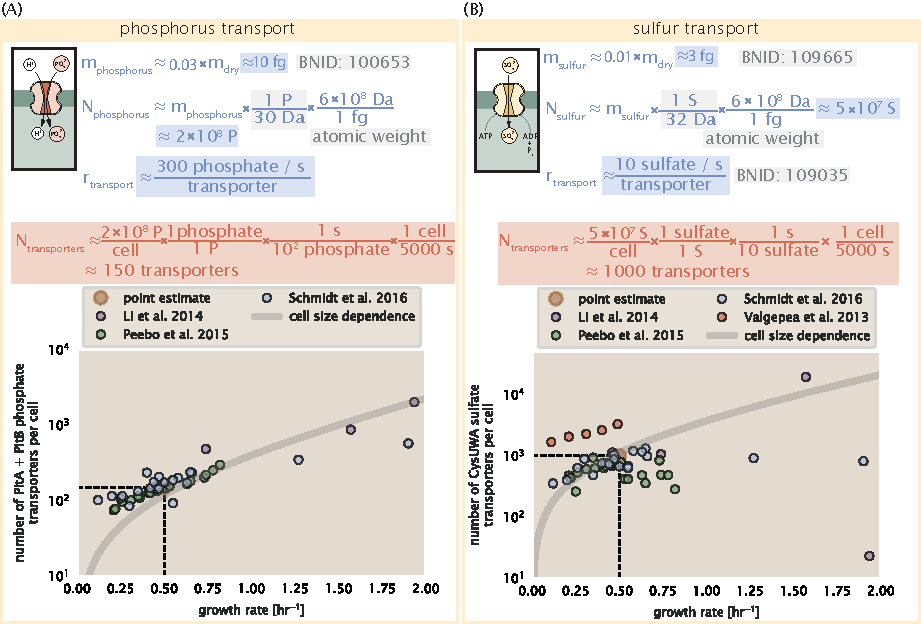
\includegraphics{main_figs/fig3_phospho_sulfo_transport.pdf}
        \caption{\textbf{Estimates and measurements of phosphate and sulfate
        transport systems as a function of growth rate.} (A) Estimate for the
        number of PitA phosphate transport systems needed to maintain a 3\%
        phosphorus \textit{E. coli} dry mass. Points in plot correspond to the
        the total number of PitA transporters per cell. (B) Estimate of the
        number of CysUWA complexes necessary to maintain a 1\% sulfur \textit{E.
        coli} dry mass. Points in plot correspond to average number of CysUWA
        transporter complexes that can be formed given the transporter
        stoichiometry [CysA]$_2$[CysU][CysW][Sbp/CysP].}
        \label{fig:phospho_sulfo_tport}
    }
    \end{fullwidth}
\end{figure*}

\subsection{Nitrogen Transport}
Finally, we turn to nitrogen transport as the last remaining transport system
highlighted in \FIG{categories}. Unlike phosphate, sulfate, and various sugar
molecules, nitrogen in the form of ammonia can readily diffuse across the
cell membrane and has a permeability on par with water ($\approx 10^5$ nm/s,
BNID:110824 \cite{milo2010}). In particularly nitrogen-poor
conditions, \textit{E. coli} expresses a transporter (AmtB) which appears to aid in
nitrogen assimilation, though the mechanism and kinetic details of transport
is still a matter of debate \citep{heeswijk2013a, khademi2004}. Beyond ammonia,
another plentiful source of nitrogen come in the form of glutamate, which has it's
own complex metabolism and scavenging pathways. However, nitrogen is plentiful
in the growth conditions examined in this work, permitting us to neglect
nitrogen transport as a potential rate limiting process in cell division.

% \section{Energy Production}
Cells consume and generate energy predominantly in the form of nucleoside
triphosphates (NTPs) in order to grow. The high-energy phosophodiester bonds of
(primarily) ATP power a variety of cellular processes that drive biological
systems away from thermodynamic equilibrium. We now turn to the synthesis of ATP
as a potential process that may limit growth, which also requires us to consider
the maintenance of the electrochemical proton gradient which powers it.

\subsection{ATP Synthesis}
Hydrolysis of the terminal phosphodiester bond of ATP into ADP (or
alternatively GTP and GDP) and an inorganic phosphate provides the
thermodynamic driving force in a wide array of biochemical reactions. One
such reaction is the formation of peptide bonds during translation, which
requires $\approx$ 2 ATPs for the charging of an amino acid to the tRNA and
$\approx$ 2 GTPs for the formation of each peptide bond. Assuming the ATP
costs associated with error correction and post-translational modifications
of proteins are negligible, we can make the approximation that each peptide
bond has a net cost of $\approx$ 4 ATP (BNID: 101442).
Formation of GTP from ATP is achieved via the action of nucleoside
diphosphate kinase, which catalyzes this reaction without an energy
investment \citep{lascu2000} and therefore consider all NTP requirements of
the cell to be functionally equivalent to being exclusively ATP. In total,
the energetic costs of peptide bond formation consume $\approx$ 80\% of the
cells ATP budget [BNID: 107782; 106158; 101637; 111918,
\cite{lynch2015,stouthamer1973}]. The pool of ATP is produced by the
F$_1$-F$_0$ ATP synthase -- a membrane-bound rotary motor which under ideal
conditions can yield $\approx$ 300 ATP per second [BNID: 114701;
\cite{weber2003}].

To estimate the total number of ATP equivalents consumed during a cell cycle, we
will make the approximation that there are $\approx 3\times10^6$ proteins per
cell with an average protein length of $\approx$ 300 peptide bonds (BNID:
115702; 108986; 104877). Taking these values together, coupled with an estimate
of $\approx$ 4 ATP equivalents per peptide bond, we find that the typical
\textit{E. coli} cell consumes $\sim 5 \times 10^9$ ATP per cell cycle on
protein synthesis alone. Assuming that each ATP synthases operates at its
maximal speed (300 ATP per second per synthase), $\approx$ 3000 ATP synthases
are needed to keep up with the energy demands of the cell. This estimate
is comparable with the experimental observations,  shown in
\FIG{energy_production} (A). We note that this estimate assumes all ATP is
synthesized via ATP synthase and neglects synthesis via fermentative metabolism.
This simplification may explain why at the fastest growth rates ($\approx$ 2
hr$^{-1}$), our continuum estimate predicts more synthase than is experimentally
observed (gray line in \FIG{energy_production}). At rapid growth rates,
\textit{E. coli} enters a type of overflow metabolism where fermentative
metabolism becomes pronounced \citep{szenk2017}.

\subsection{Generating the Proton Electrochemical Gradient}
In order to produce ATP, the F$_1$-F$_0$ ATP synthase itself must consume
energy. Rather than burning through its own product (and violating
thermodynamics), this intricate macromolecular machine has evolved to exploit
the electrochemical potential established across the inner membrane through
cellular respiration. This electrochemical gradient is manifest by the pumping
of protons into the intermembrane space via the electron transport chains as
they reduce NADH. In \textit{E. coli}, this potential difference is $\approx
-$200 mV (BNID: 102120). A simple estimate of the inner membrane as a capacitor
with a working voltage of -200 mV reveals that $\approx 2\times 10^4$ protons
must be present in the intermembrane space. However, each rotation of an ATP
synthase shuttles $\approx$ 4 protons into the cytosol (BNID: 103390). With a few thousand ATP
synthases producing ATP at their maximal rate, the potential difference would be
rapidly abolished in a few milliseconds if it were not being actively
maintained.

The electrochemistry of the electron transport complexes of \textit{E. coli}
have been the subject of intense biochemical and biophysical study
\citep{ingledew1984, khademian2017,cox1970,henkel2014}. A recent work
\citep{szenk2017} examined the respiratory capacity of the \textit{E. coli}
electron transport complexes using structural and biochemical data, revealing
that each electron transport chain rapidly pumps protons into the
intermembrane space at a rate of $\approx$ 1500 protons per second (BIND:
114704; 114687). Using our estimate of the number of ATP synthases required
per cell [\FIG{energy_production}(A)], coupled with these recent
measurements, we estimate that $\approx 3000$ electron transport complexes
would be necessary to facilitate the $\sim 5 \times 10^6$ protons per second
diet of the cellular ATP synthases. This estimate is in agreement with the
number of complexes identified in the proteomic datasets [plot in
\FIG{energy_production}(B)]. This suggests that every ATP synthase must be
accompanied by $\approx$ 1 functional electron transport chain.

\begin{figure}
    \begin{fullwidth}
        \centering{
            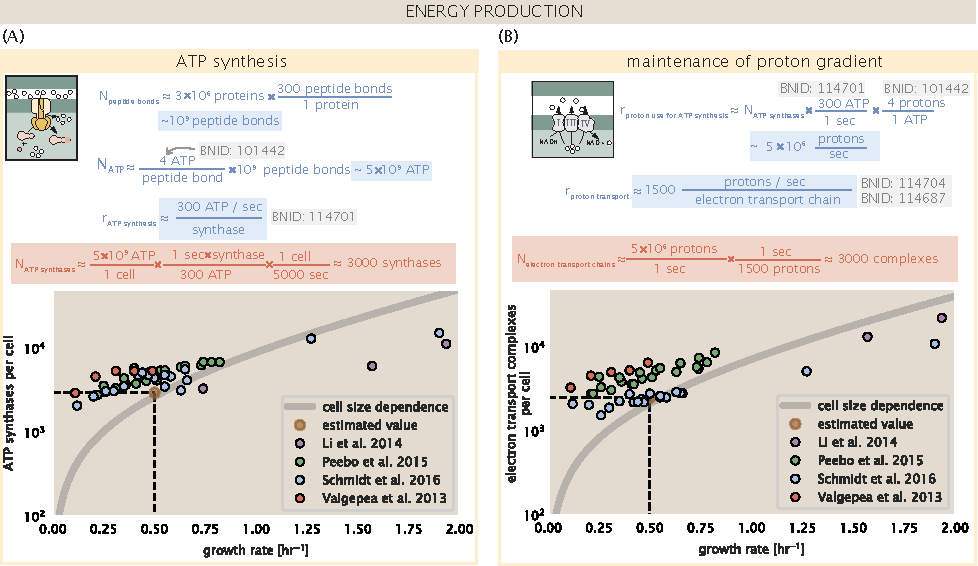
\includegraphics{main_figs/fig4_energy_production.pdf}
            \caption{\textbf{The abundance of F$_1$-F$_0$ ATP synthases and
            electron transport chain complexes as a function of growth
            rate.} (A) Estimate of the number of F$_1$-F$_0$ ATP synthase
            complexes needed to accommodate peptide bond formation and other NTP
            dependent processes. Points in plot correspond to the
            mean number of complete F$_1$-F$_0$ ATP synthase complexes that
            can be formed given proteomic measurements and the subunit
            stoichiometry
            [AtpE]$_{10}$[AtpF]$_2$[AtpB][AtpC][AtpH][AtpA]$_{3}$[AtpG][AtpD]$_3$.
            (B) Estimate of the number of electron transport chain complexes
            needed to maintain a membrane potential of $-$200 mV given
            estimate of number of F$_1$-F$_0$ ATP synthases from (A). Points
            in plot correspond to the average number of complexes identified
            as being involved in aerobic respiration by the Gene Ontology
            identifier GO:0019646 that could be formed given proteomic
            observations. These complexes include cytochromes \textit{bd1}
            ([CydA][CydB][CydX][CydH]), \textit{bdII} ([AppC][AppB]),
            \textit{bo$_3$},([CyoD][CyoA][CyoB][CyoC]) and NADH:quinone
            oxioreducase I
            ([NuoA][NuoH][NuoJ][NuoK][NuoL][NuoM][NuoN][NuoB][NuoC][NuoE][NuoF][NuoG][NuoI])
            and II ([Ndh]). Grey lines in both (A) and (B) correspond to the
            estimate procedure described, but applied to a continuum of growth
            rates. We direct the reader to the Supporting Information for a more
            thorough description of this approach.}
        \label{fig:energy_production}
        }
    \end{fullwidth}
\end{figure}


\subsubsection{Limits on Biosynthesis in a Crowded Membrane}
Our estimates thus far have focused on biochemistry at the periphery of the cell.
Since surface area and volume do not scale identically as cell size changes,  in
order to better understand the physical constraints on transport and  energy
production it is necessary to consider the consequence of a changing S/V
ratio, which will decrease at faster growth rates. Here we use our analysis of
ATP production  to consider this constraint.

In our estimate of ATP production above we found that a cell demands about $5
\times 10^9$ ATP per cell cycle or $10^6$ ATP/s. With a cell volume of roughly 1
fL (BNID: 100004), this corresponds to about $2 \times 10^{10}$ ATP per fL of cell volume, in
line with previous estimates \citep{stouthamer1977, szenk2017}. In
\FIG{energy_scaling} (A) we plot this ATP demand as a function of the S/V ratio
in green, where we have considered a range of cell shapes from spherical to
rod-shaped with an aspect ratio (length/width) equal to 4. In order to consider
the maximum ATP that could be produced, we consider the amount of ATP that can
be generated by a membrane filled with ATP synthase and electron transport
complexes and a maximal production rate of about 3 ATP / (nm$^2 \cdot$s)
\citep{szenk2017}. This is shown in blue in \FIG{energy_scaling}(A), which shows
that at least for the growth rates observed (right column in plot), the energy
demand is roughly an order of magnitude less. Interestingly, \cite{szenk2017}
found that ATP production by respiration is less efficient than by
fermentation on a per membrane area basis, due to the additional proteins of the
electron transport chain. This suggests that, even under anaerobic growth, cells
will have sufficient membrane space for ATP production.

The analysis highlights that there will indeed be a maximum attainable cell size
due to a diminishing capacity to provide resources as the cell increases in
size. The maximum energy production in \FIG{energy_scaling}(A), however, does
represent a somewhat unachievable limit since the inner membrane must also
include other proteins such as those we've considered for nutrient transport and cell
wall biogenesis. To better understand the overall proteomic makeup of the inner
membrane, we therefore used Gene Ontology (GO) annotations \citep{ashburner2000,
thegeneOntologyconsortium2018} to identify all proteins embedded or peripheral
to the inner membrane (GO term: 0005886). Those associated but not
membrane-bound include proteins like MreB and FtsZ and must nonetheless be
considered as a vital component occupying space on the membrane. In
\FIG{energy_scaling}(B), we find that the total protein mass per \textmu m$^2$
is nearly constant across growth rates. Interestingly, when we consider the
distribution of proteins grouped by their Clusters of Orthologous Groups (COG)
\citep{tatusov2000}, the relative abundance for those in metabolism (including
ATP synthesis via respiration) is also relatively constant across growth rates,
suggesting that no one process (energy production, nutrient uptake, etc.) is
particularly dominating even at fast growth rates [\FIG{energy_scaling}(C)].

\begin{figure}
    \begin{fullwidth}
        \centering{
            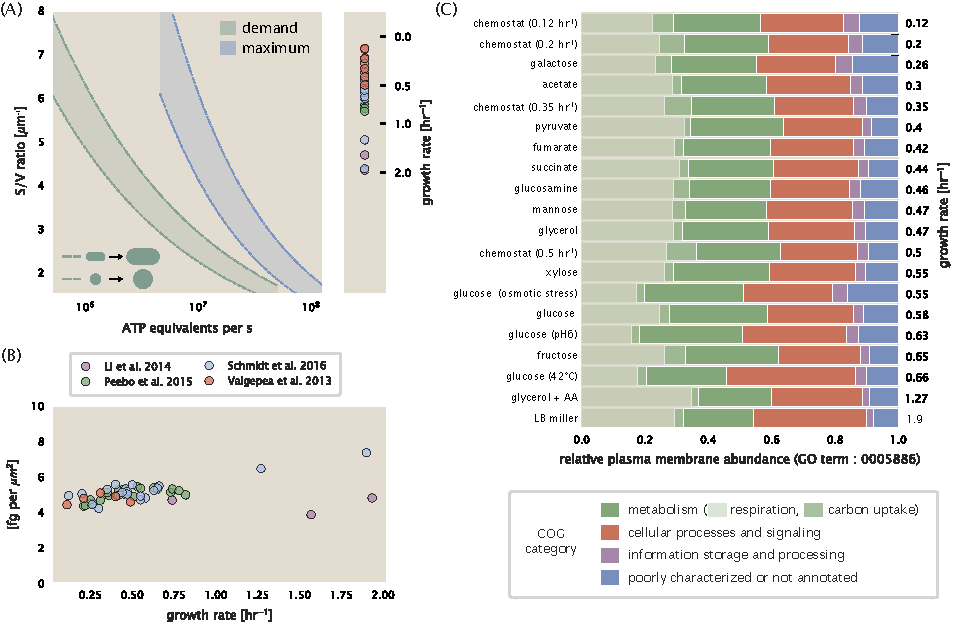
\includegraphics{main_figs/fig5_energy_SV_scaling.pdf}
            \caption{\textbf{Influence of cell size and surface area to volume
            (S/V) ratio on ATP production and inner membrane composition.} (A) Scaling
            of ATP demand and maximum ATP production through respiration as a
            function of S/V ratio. Cell volumes of 0.5 fL to 50 fL were
            considered, with the dashed (\texttt{- -}) line corresponding to a
            sphere and the dash-dot line (\texttt{-.}) reflecting a rod-shaped
            bacterium like \textit{E. coli} with a typical aspect ratio (length
            / width) of 4 \citep{shi2018}. The ATP demand is calculated as
            $10^6$ ATP/(\textmu m$^3$ s), while the maximum ATP production rate
            is taken to be 3 ATP / (nm$^2 \cdot$s)
            \citep{szenk2017}, with calculations of \textit{E. coli} volume and
            surface area detailed in Appendix \nameref{sec:protein_size_SV}. In
            this calculation, 50\% of the bacterial inner membrane is assumed to
            be protein, with the remainder lipid. (B) Total protein mass per
            \textmu m$^2$ calculated for proteins with inner membrane annotation
            (GO term: 0005886). (C) Relative protein abundances by mass based on
            COG annotation. Metabolic proteins are further separated into
            respiration (F$_1$-F$_0$ ATP synthase, NADH dehydrogenase I,
            succinate:quinone oxidoreductase, cytochrome bo$_3$ ubiquinol
            oxidase, cytochrome bd-I ubiquinol oxidase) and carbohydrate
            transport (GO term: GO:0008643). Note that the elongation factor
            EF-Tu can also associate with the inner membrane, but was excluded
            in this analysis due to its high relative abundance (roughly
            identical to the summed protein shown in part
            (B)).}\label{fig:energy_scaling}
            }
                \end{fullwidth}
\end{figure}



% \begin{table}[bt]
% \caption{\label{tab:example}Automobile Land Speed Records (GR 5-10).}
% % Use "S" column identifier to align on decimal point 
% \begin{tabular}{S l l l r}
% \toprule
% {Speed (mph)} & Driver          & Car                        & Engine    & Date     \\
% \midrule
% 407.447     & Craig Breedlove & Spirit of America          & GE J47    & 8/5/63   \\
% 413.199     & Tom Green       & Wingfoot Express           & WE J46    & 10/2/64  \\
% 434.22      & Art Arfons      & Green Monster              & GE J79    & 10/5/64  \\
% 468.719     & Craig Breedlove & Spirit of America          & GE J79    & 10/13/64 \\
% 526.277     & Craig Breedlove & Spirit of America          & GE J79    & 10/15/65 \\
% 536.712     & Art Arfons      & Green Monster              & GE J79    & 10/27/65 \\
% 555.127     & Craig Breedlove & Spirit of America, Sonic 1 & GE J79    & 11/2/65  \\
% 576.553     & Art Arfons      & Green Monster              & GE J79    & 11/7/65  \\
% 600.601     & Craig Breedlove & Spirit of America, Sonic 1 & GE J79    & 11/15/65 \\
% 622.407     & Gary Gabelich   & Blue Flame                 & Rocket    & 10/23/70 \\
% 633.468     & Richard Noble   & Thrust 2                   & RR RG 146 & 10/4/83  \\
% 763.035     & Andy Green      & Thrust SSC                 & RR Spey   & 10/15/97\\
% \bottomrule
% \end{tabular}

% \tabledata{This is a description of a data source.}

% \end{table}







% For a half-width figure or table with text wrapping around it, use 

% \begin{verbatim}
% \begin{wrapfigure}{l}{.46\textwidth}
%   \includegraphics[width=\hsize]{...}
%   \caption{...}\label{...}
% \end{wrapfigure}
% \end{verbatim}
% %
% as in \FIG{halfwidth}. For tables:

% If you use the following prefixes for your \verb|\label|:
% %
% \begin{description}
% \item[Figures] \texttt{fig:}, e.g.~\verb|\label{fig:view}|
% \item[Figure Supplements] \texttt{figsupp:}, e.g.~\verb|\label{figsupp:sf1}|\\
% (we'll assume \texttt{figsupp:sf1} is a figure supplement of \texttt{fig:view} in our example)
% \item[Figure source data] \texttt{figdata:}, e.g.~\verb|\label{figdata:first}|
% \item[Videos] \texttt{video:}, e.g.~\verb|\label{video:mv1}|
% \item[Video supplements] \texttt{videosupp:}, e.g.~\verb|\label{videosupp:sv1}|
% \item[Tables] \texttt{tab:}, e.g.~\verb|\label{tab:example}|
% \item[Equations] \texttt{eq:}, e.g.~\verb|\label{eq:CLT}|
% \item[Boxes] \texttt{box:}, e.g.~\verb|\label{box:simple}|
% \end{description}
% %
% you can then use the convenience commands \verb|\FIG{view}|, \verb|\FIGSUPP[view]{sf1}|, \verb|\TABLE{example}|, \verb|\EQ{CLT}|, \verb|\BOX{simple}|, \verb|\FIGDATA[view]{first}|, \verb|\VIDEO{mv1}| and \verb|{\VIDEOSUPP}[view]{sv1}| \emph{without} the label prefixes, to generate cross-references \FIG{view}, \FIGSUPP[view]{sf1},  \TABLE{example}, \EQ{CLT}, \BOX{simple}, \FIGDATA[view]{first}, \VIDEO{mv1} and \VIDEOSUPP[view]{sv1}. Alternatively, use \verb|\autoref| with the full label, e.g.~\autoref{first:app} (although this may not work correctly for figures and tables in the appendices or boxes nor supplements at present).

% Really wide figures or tables, that take up the entire page, including the gutter space: use \verb|\begin{fullwidth}...\end{fullwidth}| as in \FIG{fullwidth}. And sometimes you may want to use feature boxes like \BOX{simple}.

% \begin{wrapfigure}{l}{.46\textwidth}
% 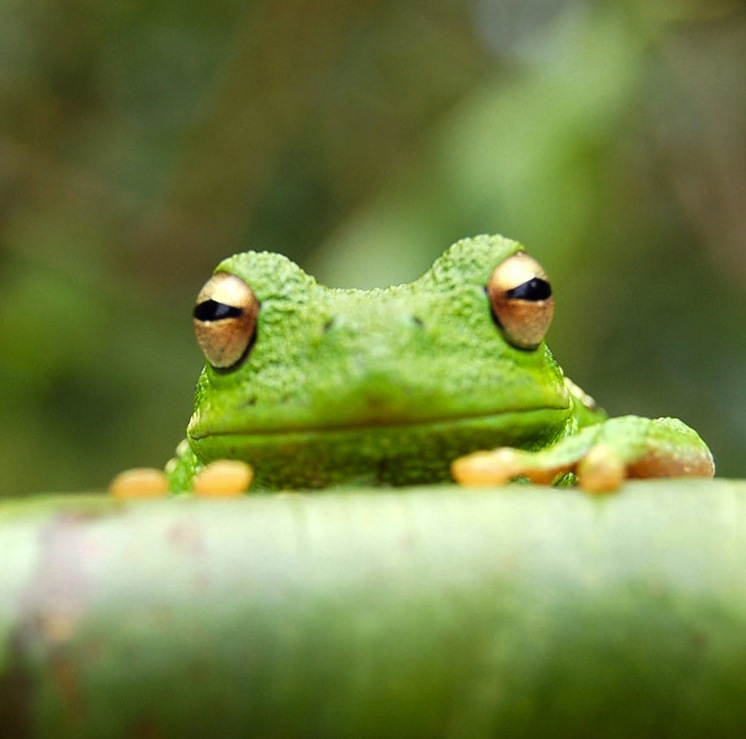
\includegraphics[width=\hsize]{frog}
% \caption{A half-columnwidth image using wrapfigure, to be used sparingly. Note that using a wrapfigure before a sectional heading, near other floats or page boundaries is not recommended, as it may cause interesting layout issues. Use the optional argument to wrapfigure to control how many lines of text should be set half-width alongside it.}
% \label{fig:halfwidth}
% \end{wrapfigure}


% \begin{figure}
% \begin{fullwidth}
% 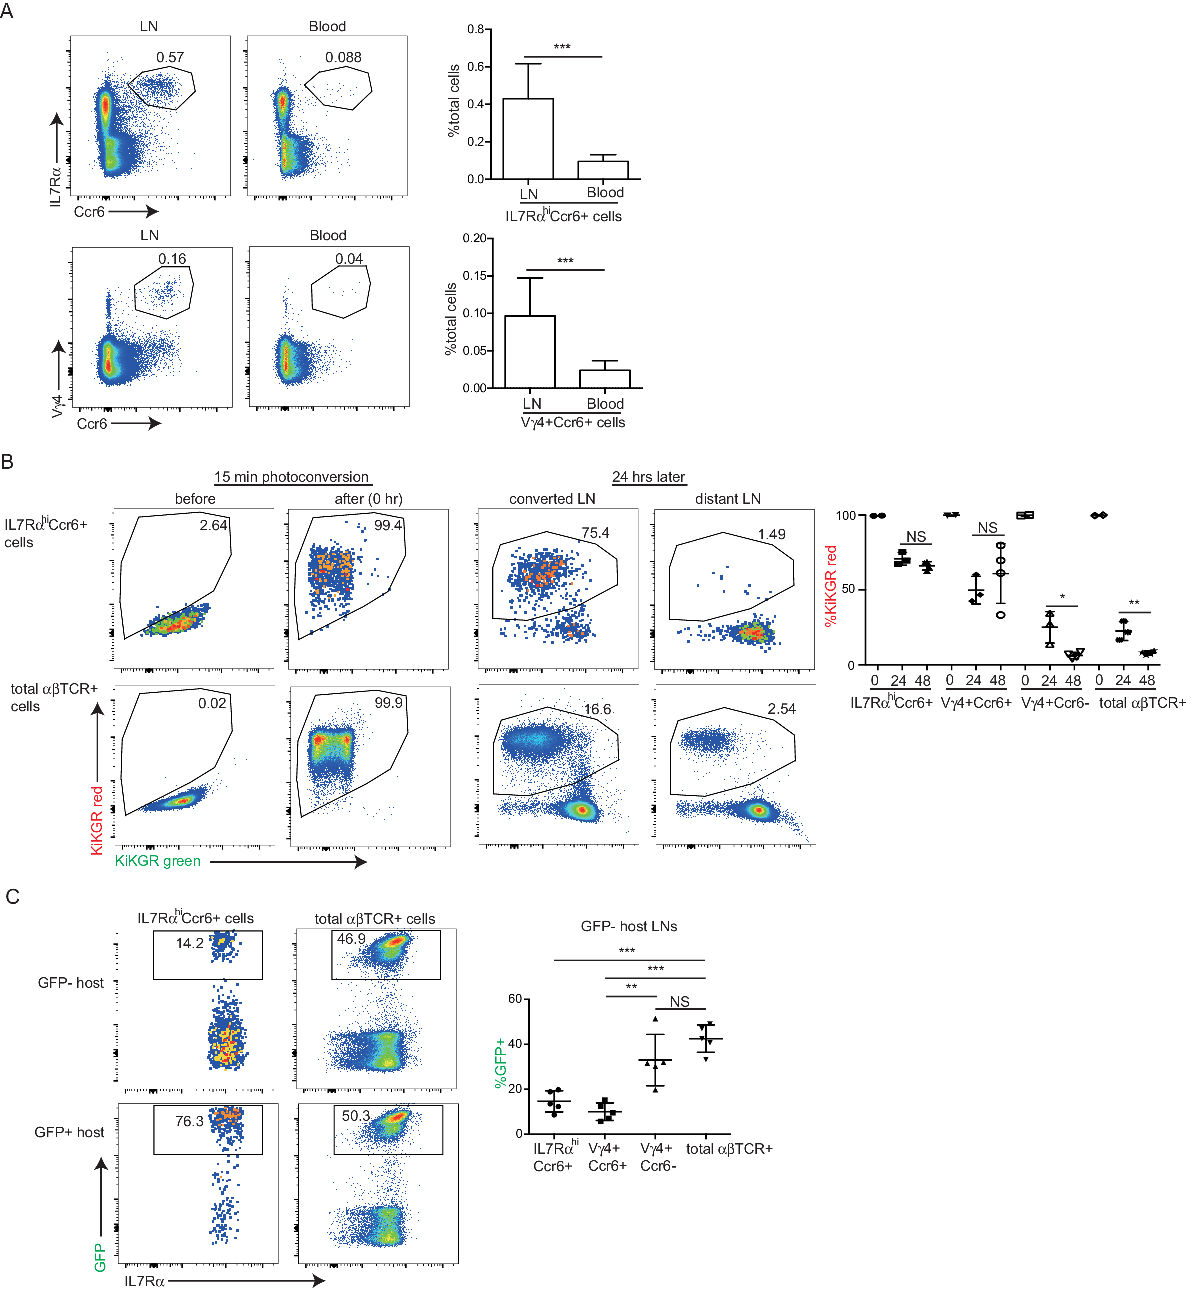
\includegraphics[width=0.95\linewidth]{elife-18156-fig2}
% \caption{A very wide figure that takes up the entire page, including the gutter space.}
% \label{fig:fullwidth}
% \figsupp{There is no limit on the number of Figure Supplements for any one primary figure. Each figure supplement should be clearly labelled, Figure 1--Figure Supplement 1, Figure 1--Figure Supplement 2, Figure 2--Figure Supplement 1 and so on, and have a short title (and optional legend). Figure Supplements should be referred to in the legend of the associated primary figure, and should also be listed at the end of the article text file.}{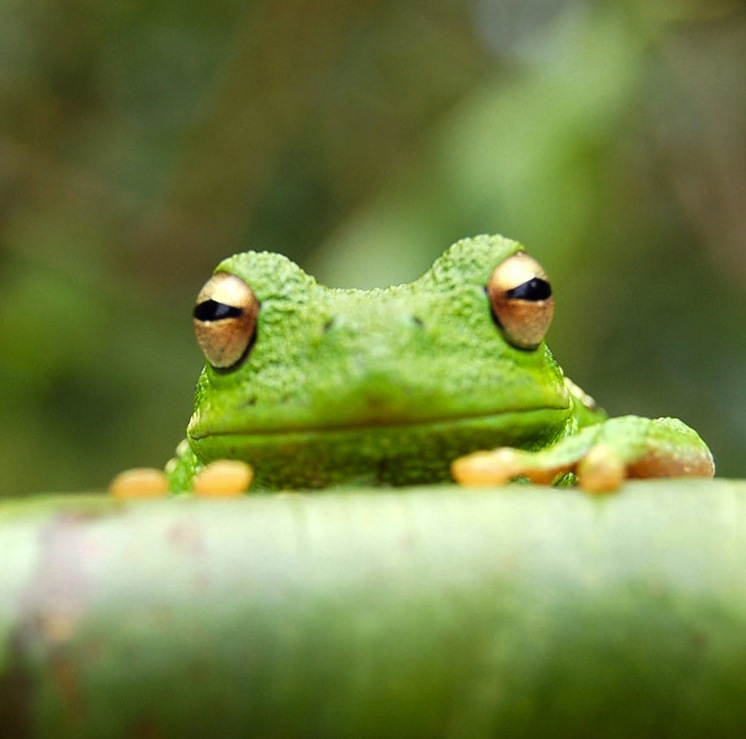
\includegraphics[width=5cm]{frog}}
% \end{fullwidth}
% \end{figure}


% \figsupp[Shorter caption for main text.]{This is a supplementary figure's full caption, which will be used at the end of the manuscript.}{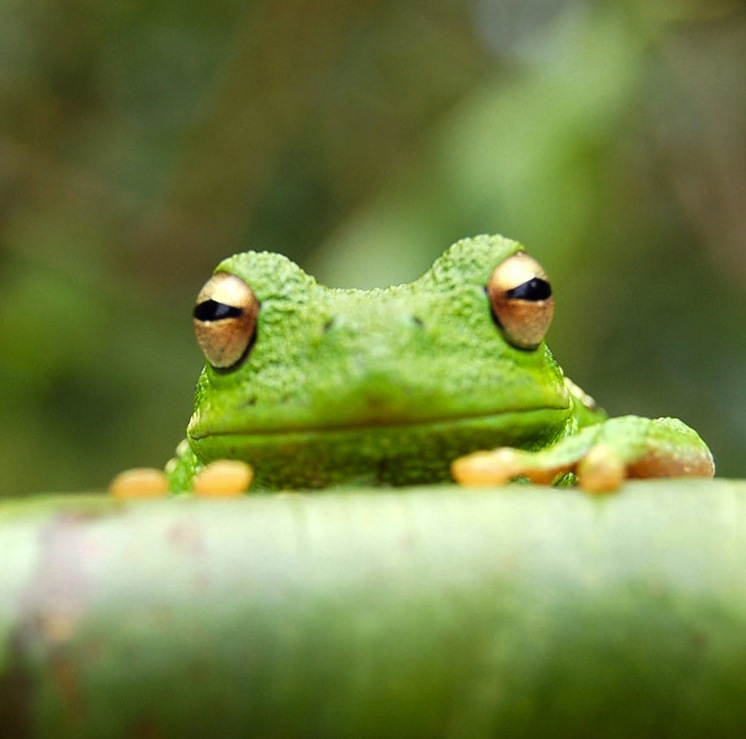
\includegraphics[width=6cm]{frog}}\label{figsupp:sf1}
% \figsupp{This is another supplementary figure.}{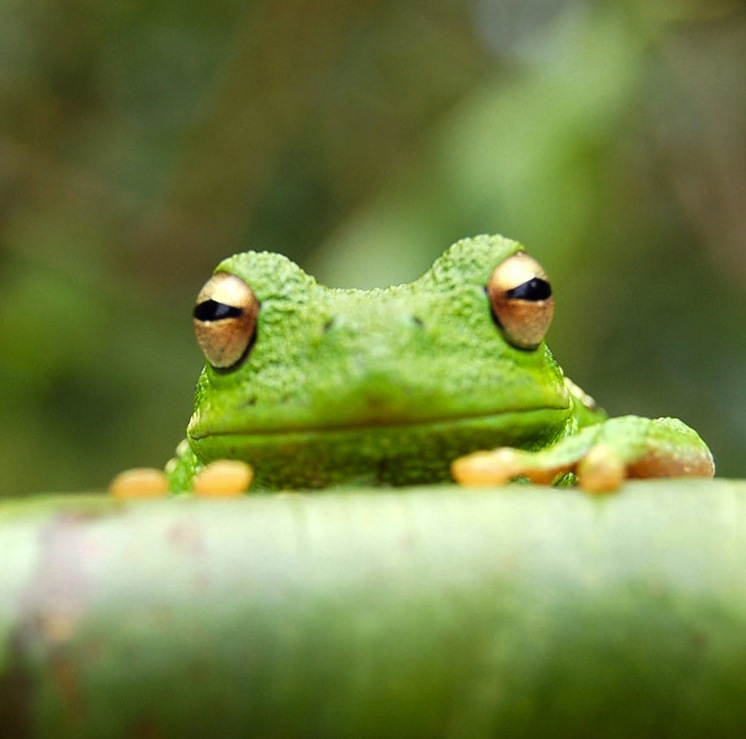
\includegraphics[width=6cm]{frog}}
% \videosupp{This is a description of a video supplement.}\label{videosupp:sv1}
% \figdata{This is a description of a data source.}\label{figdata:first}
% \figdata{This is another description of a data source.}\label{figdata:second}






% \section{Acknowledgments}

% Additional information can be given in the template, such as to not include funder information in the acknowledgments section.

% \nocite{*} % This command displays all refs in the bib file. PLEASE DELETE IT BEFORE YOU SUBMIT YOUR MANUSCRIPT!
\bibliography{library.bib}

%%%%%%%%%%%%%%%%%%%%%%%%%%%%%%%%%%%%%%%%%%%%%%%%%%%%%%%%%%%%
\end{document}